\documentclass[reprint, superscriptaddress]{revtex4-1}

\usepackage{xparse}
\usepackage{xfrac}
\usepackage{graphicx}
\usepackage{mathtools}

\usepackage{paralist}

%\usepackage{wrapfig}
\usepackage{caption}
\usepackage{threeparttable}
\usepackage{multirow}

\usepackage{url}
%\usepackage{hyperref}

\DeclareDocumentCommand{\CS}{sO{}}{\IfBooleanTF{#1}{\hat{\sigma}_{#2}}{\sigma_{#2}}}
\DeclareDocumentCommand{\slp}{sO{}}{\IfBooleanTF{#1}{\hat{\beta}_{#2}}{\beta_{#2}}}
\DeclareDocumentCommand{\Thick}{O{}}{\Theta_{#1}}

\DeclareDocumentCommand{\SE}{sm}{\IfBooleanTF{#1}{\hat{\sigma}\bkt*{#2}}{\sigma\bkt*{#2}}}

\DeclareDocumentCommand{\bkt}{sm}{\IfBooleanTF{#1}{\left[ #2 \right]}{\left(#2\right)}}
\newcommand{\td}{\mathrm{d}}

\DeclareDocumentCommand{\ADCcode}{O{ }}{unit{#1}}

\newcommand{\scl}{.4}

\DeclareDocumentCommand{\Ayy}{s}{\IfBooleanT{#1}{\hat}A_{y,y}}
\DeclareDocumentCommand{\Ayxz}{s}{\IfBooleanT{#1}{\hat}A_{y,xz}}

\newcommand{\vp}[2]{#1\cdot10^{#2}}

\begin{document}
\title{Preparation for the Time Reversal Invariance experiment at COSY (TRIC)}
\author{Aleksandr Aksentev}
\affiliation{National Research Nuclear University ``MEPhI,'' Kashirskoe shosse, 31, Moscow, Russia, 115409}
\affiliation{Forschungszentrum J\"ulich GmbH, Leo-Brandt-Straße,	52428 J\"ulich, Germany}
\author{Dieter Eversheim}
\affiliation{Helmholtz-Institut f\"ur Strahlen- und Kernphysik der Universit\"at Bonn, Nussallee 14-16, 53115 Bonn, Germany}
\author{Berndt Lorentz}
\affiliation{Forschungszentrum J\"ulich GmbH, Leo-Brandt-Straße,	52428 J\"ulich, Germany}
\author{Yury Valdau}
\affiliation{Helmholtz-Institut f\"ur Strahlen- und Kernphysik der Universit\"at Bonn, Nussallee 14-16, 53115 Bonn, Germany}

\maketitle

\captionsetup[figure]{labelfont=bf,textfont=normalfont,singlelinecheck=off,justification=raggedright}

	
	
\begin{abstractname}
 In this contribution we describe a possible procedure for estimating the effective total unpolarized cross section and cross section asymmetry from measurements of average beam current. We also present the estimates obtained for the cross sections $\CS[0]^{pp}$ and $\CS[0]^{pd}$ in the cases of $pp$ and $pd$ scattering, as well as the asymmetry $\Ayy$ in double-polarized $\vec{p}\vec{d}$ scattering, from data collected in September 2012 and June 2016 at the cooler synchrotron COSY-J\"ulich in the course of a preliminary experiment to the test of Time-Reversal Invariance at COSY (TRIC). 
\end{abstractname}

\section{TRIC Experiment}

TRIC (test of Time-Reversal Invariance at COSY) is a transmission experiment planned at the COoler SYnchrotron COSY-J\"ulich for the purpose of testing Time-Reversal Invariance. Its physical foundation is the use of a genuine null-observale for T-symmetry, --- the total cross section asymmetry in double-polarized proton-deuteron scattering, --- whose existence is guaranteed by the optical theorem~\cite{Conzett}. TRIC is aimed at achieving the accuracy of $10^{-6}$ in the cross section asymmetry estimate $\Ayxz*$.

The total cross section in a double-polarized scattering involves a number of polarization-dependent terms:
\begin{equation}\label{eq:PolCS}
	\CS[tot] = \CS[0]\cdot\bkt{1 + \sum_{i,j} A_{i,j} P_iP^t_j + \sum_{k, mn} A_{k,mn}P_k P^t_{mn}},
\end{equation}
where $P^t_j$ and $P_i$ are respectively the $j$-projection of target and the $i$-projection of beam polarizations, $P^t_{mn}$ is the $mn$-tensor component of target polarization, $\CS[0]$ is the unpolarized cross section component, and $A_{i,j}$/$A_{k,mn}$ is the appropriate asymmetry.

The asymmetry that serves as the null-observable of T-symmetry is $A_{y,xz}$, all others being faking observables~\cite{Conzett}. TRIC's experimental design limits the influence of all faking observables to below the experimental accuracy ~\cite{Proposal}, except for that of $A_{y,y}$, caused by the misalignment of the target and beam polarizations. Thus arises the problem of knowing the extent to which vector target polarization must be controlled, for which the knowledge of the value of $A_{y,y}$ is required. 

Unpolarized cross section $\CS[0]$ is a parameter in both estimators' distributions, and hence it must be known as well. 

In this proceeding we summarize the results of two experiments preliminary to TRIC, in order to assess the viability of the transmission-experiment-based method of accessing the $\Ayxz$ observable.

\section{Theoretical background}
\subsection{Physics}
The intensity of a particle beam revolving inside an accelerator decreases according to the Beer-Lambert law:
\begin{align*}
	I_{n+1} &= I_n \cdot \exp\bkt{-\sum_{i=i}^N \CS[i]\cdot\int_0^L n_i(z)\td z} \\
			&= I_n \cdot \exp\bkt{-\sum_{i=i}^N \CS[i]\cdot \Thick[i]} \\
			&= I_n \cdot \exp\bkt{-\sum_i\frac1\tau_i},
\end{align*}
where $L$ is the beam path length, $N$ is the number of attenuating species, $\CS[i]$ is the attenuation cross section, $n$ is the number of passed revolutions, $\Thick[i] = \int_L n_i(z)\td z$ is the thickness of the corresponding attenuating element.

For the average beam current, integration of the above yields
\begin{equation}\label{eq:CurrentDecay}
	I_t = I_0 \cdot \exp\bkt{\slp\cdot t},
\end{equation}
with $\slp = \sum_i \slp[i] = - \nu\cdot\sum_i \sfrac1\tau_i$, $\nu$ --- the beam revolution frequency. 

In the case of unpolarized scattering, an unpolarized beam interacts with an unpolarized gas target with cross section $\CS[0]$; to that add all the losses in the accelerator ring ($\CS[x]\Thick[x]$), to produce the following expression for beam loss:
\begin{equation}\label{eq:SlopeModel}
	\slp = -\nu\bkt{\CS[0]\Thick + \CS[x]\Thick[x]}.
\end{equation}

Since $\CS[x]\Thick[x]$ is independent from the presence of the target, an estimate of the cross section is obtained from  
\begin{equation}
	\CS*[0] = \frac{\slp*[off] - \slp*[on]}{\nu\Thick[on]},
\end{equation}
where $\slp*[on/off]$ is the slope estimate in an on-/off-cycle.

In the $pd$ scattering in which both the beam and the target have vector polarization, from equation~\eqref{eq:PolCS}, beam loss is
\[
	\slp = -\nu\bkt{\CS[0](1 + \Ayy P_y^t P_y)\Thick[on] + \CS[x]\Thick[x]},
\]
from which an asymmetry estimate can be computed as the difference between the slopes with spin states \emph{up} and \emph{down}:
\begin{equation}\label{eq:AyyEst}
	\Ayy* = \frac{\slp*[on]^- - \slp*[on]^+}{\nu P_y^t\Delta P_y\cdot \CS[0]\Thick[on]}.
\end{equation}

\subsection{Statistics}

We estimate $\slp$ by fitting a linear model to logarithmized beam current data, $\ln I_t = \ln I_0 + \slp\cdot t + \epsilon_t$, using the least squares method. In order that the estimate be minimum-variance mean-unbiased, the data must satisfy the Gauss-Markov conditions: %~\cite{GaussMarkov}
\begin{enumerate}
	\item Linearity and additivity of the relationship;
	\item Independence of the time and error variables (strict exogeneity);
	\item No serial correlation of the error;
	\item Constant variance of the error (homoskedasticity).
\end{enumerate}

Linearity is necessary for the validity of using linear regression; homoskedasticity and absence of serial correlation are required for the efficiency, and exogeneity for the consistency of the estimator.

This means the following series of questions has to be answered in order to verify the validity of our results:
\begin{enumerate}
	\item Is the logarithm of beam current a linear function of time?
	\item Are the errors uncorrelated with time?
		\begin{itemize}
			\item Is measurement time measured with negligible error?
			\item Are there predictors other than time?
			\item Is there among the omitted variables a predictor dependent on current?
		\end{itemize}
	\item What is the interpretation of the slope?
\end{enumerate}

Below, we will be concerned with the former two.

\section{Overview of data}
We have analyzed two data sets: one was measured in 2012, the other in 2016. 

In the 2012 experiment, the proton beam was scattered on the hydrogen target, both unpolarized; the beam was cooled using electron cooling and bunched by the barrier bucket; the cycles lasted for one hour each. 

In the 2016 experiment the proton beam was scattered on the deuteron target, both polarized; the beam had undergone RF-bunching and electron-cooling; the cycles lasted for 12 minutes, the first half of which the target was turned on, in the second off; the beam spin state alternated from spin up to spin down through no spin, while the target spin state remained constant (spin up). 

In both experiments the target was produced by an Atomic Beam Source (ABS) capable of producing jets of polarized hydrogen and deuterium, and was concentrated within a storage cell located inside the PAX target chamber, described in more detail in~\cite{Weidemann}. The cycles for both experiments are presented in FIG.~\ref{fig:Cycles}. The measurements were made with a Bergoz Beam Current Transformer, and read out by a Siemens ADC (Simatic S7 6ES7331-7KF01-0AB0). In the 2012 experiment, the BCT offset was around 2300 a.u., in 2016, the offset it was about 4300 a.u. The zeroing of current before each cycle, that can be observed in the 2012 panel, is due to the overflow of the measurement system, since the beam current at injection lead to a voltage that is out of range for this ADC.

\begin{figure}[h]
	\centering
	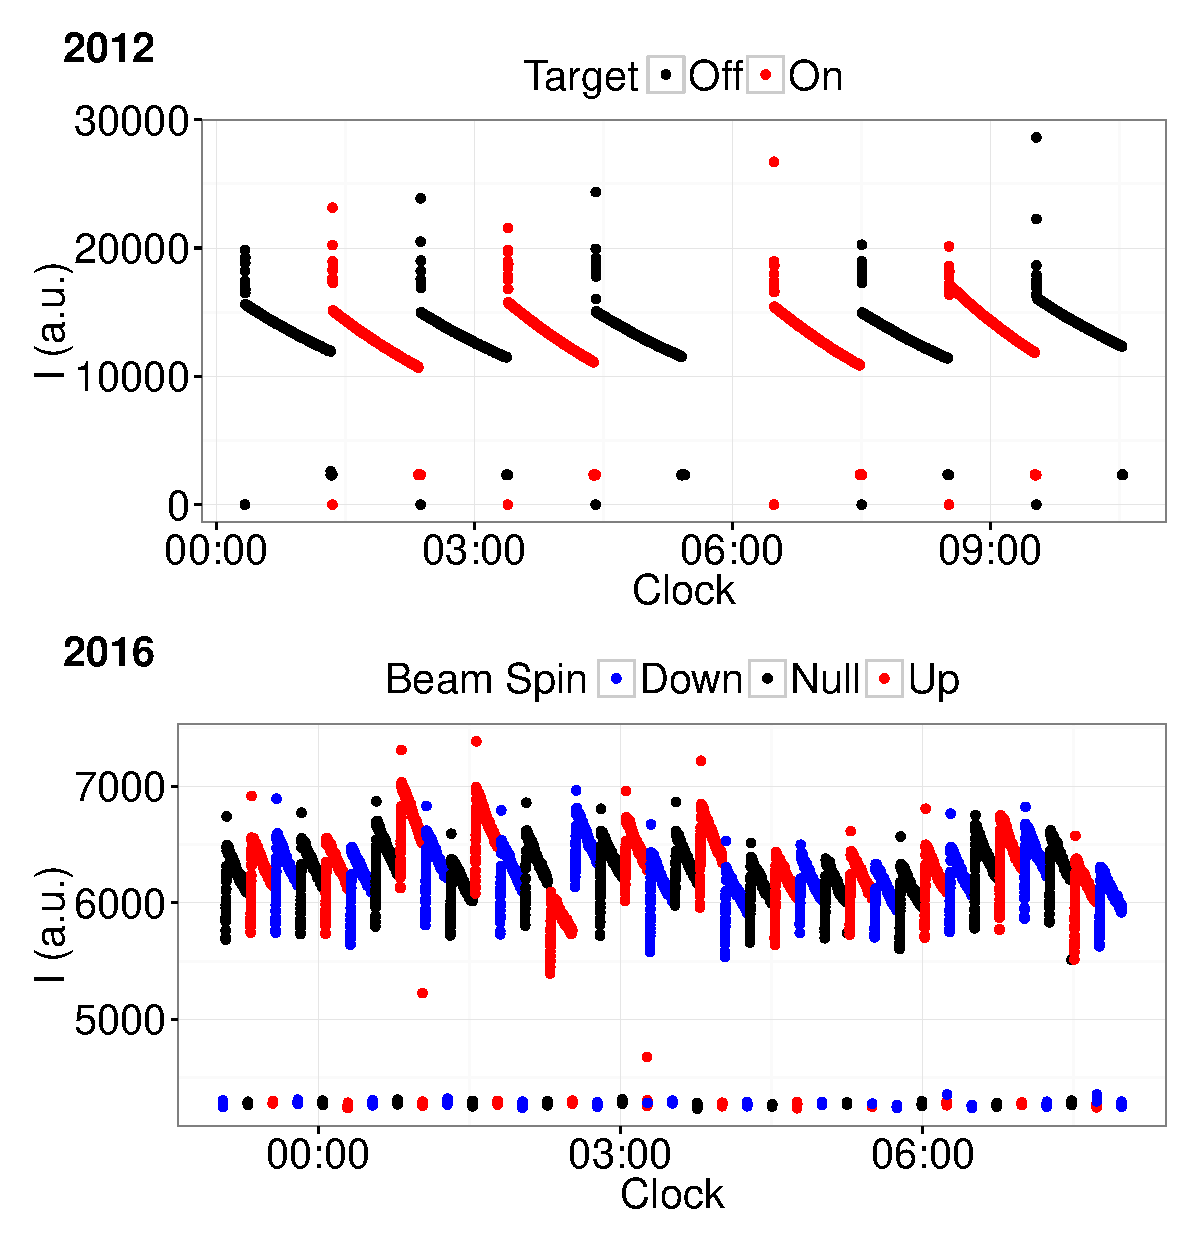
\includegraphics[scale=\scl]{img/Cycles_12--16.eps}
	\caption{Average beam current as a function of time. Upper panel: experiment in 2012; the cycles with the target present are drawn in red, those without in black. Lower panel: experiment in 2016. The cycles are colored according to the beam spin state (red for spin up, blue for down, and black for cycles with unpolarized beam). The first half of a cycle is collected with the target turned on, the second half off.~\label{fig:Cycles}}
\end{figure} 


\section{Slope}\label{sec:Slope}

In order to correctly estimate a cycle's slope, we subtract the BCT offset $\Delta$ from the data. This is done  because slope
\begin{align*}
	\tilde{\slp} &= \frac{\td\ln \tilde{I}_t}{\td t} 
				  = \frac{1}{\tilde{I}_t}\frac{\td \tilde{I}_t}{\td t}, 
\shortintertext{where, if the measured current}
	\tilde{I}_t  	&= I_t + \Delta_t = I_0\exp\bkt{\slp\cdot t} + \Delta_t, 
\shortintertext{then}
\tilde{\slp} 	&= \frac{1}{1 + \lambda_t}\bkt{\slp + \frac1{I_t}\frac{\td\Delta_t}{\td t}}, \\
	\lambda_t	&= {I_0}^{-1}\cdot \Delta_t\cdot\exp\bkt{-\slp\cdot t}.
\end{align*}

Even a constant offset must be removed in order to have a constant slope to estimate. The presence of an offset (let alone a time-dependent one) violates the exogeneity assumption, and hence biases the estimate. At this stage, estimation was done assuming offset was constant within a cycle, and its value was estimated as the median of the post-cycle current.

\begin{table}
\centering
\begin{threeparttable}
	\caption{Characteristics of a typical cycle.\label{tbl:CycleChars}}
	\begin{tabular}{llr}
	\hline\hline
	Charactetistic	& Test 					& P-value\\
	\hline
	Linearity 		& Harvey-Collier		& 0\% \\
	-				& Rainbow				& 0\% \\
	Constant slope	& Chow\tnote{a}		 	& 100\% \\
	-				& Moving estimates		& 1\% \\
	Homoskedasticity& Breusch-Pagan 		& 0\% \\
	Autocorrelation & Durbin-Watson			& 0\% \\
	\hline\hline
	\end{tabular}
	\begin{tablenotes}
		\item[a]{The Chow test was performed at every point in the fitting range. The average of F-statistics is used as the test statistic.}
	\end{tablenotes}
\end{threeparttable}
\end{table}

After subtracting the offset, the linear model $\ln I_t = \ln I_0 + \slp t +\epsilon_t$ is fitted via the ordinary least squares method. The reduced chi-squares computed from model residuals deviate from one starting from the fourth decimal place; however, one should note that the data are likely to have structural slope changes, and do not pass linearity tests as well (see TABLE~\ref{tbl:CycleChars}). Because the model residuals exhibit serial correlation (FIG.~\ref{fig:Run969}), the slope estimates' standard errors are estimated with robust estimators. This procedure is applied to both data sets.

\newcommand{\avg}[1]{\langle #1 \rangle}
The fit results for all the slopes are summarized in TABLE~\ref{tbl:Slp-big}. The results contradict our expectations, because, for target-on slopes, the effective cross section is expected to increase when the beam spin is up, and decrease when it's down, i.e. $\slp^+ < \slp^0 < \slp^-$; the estimates, however, satisfy $\slp*^0 < \slp*^- < \slp*^+$. This might have suggested that the labeling of the spin states was done incorrectly. 

We checked this hypothesis by using the pull distribution $p(a,b) = \frac{\avg{a}-\avg{b}}{\sqrt{\SE{a}^2+\SE{b}^2}}$, and testing whether the sample means are different depending on the beam spin state. The conclusion is that they are not (the T-test P-values are: 72\% (Up-Down), 73\% (Up-Null), 47\% (Null-Down)); for this reason, we assume that the spin states are labeled correctly.

\begin{threeparttable}[h]
	\centering
	\caption{Slope summary statistics. \label{tbl:Slp-big}}
	\begin{tabular}{c|llrllrr}
		\hline\hline
		        Year          & Target               & Spin & \#\tnote{a} & Mean [a.u.]      & SE [a.u.]    &  \\ \hline
		\multirow{2}{*}{2012} & Off                  & Null & 5           & $\vp{-9.04}{-5}$ & $\vp{6}{-7}$ &  \\
		                      & On                   & Null & 4           & $\vp{-1.20}{-4}$ & $\vp{1}{-6}$ &  \\ \hline
		\multirow{6}{*}{2016} & \multirow{3}{*}{Off} & Up   & 12          & $\vp{-2.26}{-4}$ & $\vp{7}{-6}$ &  \\
		                      &                      & Down & 12          & $\vp{-2.16}{-4}$ & $\vp{8}{-6}$ &  \\
		                      &                      & Null & 12          & $\vp{-2.12}{-4}$ & $\vp{9}{-6}$ &  \\
		                      & \multirow{3}{*}{On}  & Up   & 12          & $\vp{-2.51}{-4}$ & $\vp{4}{-6}$ &  \\
		                      &                      & Down & 12          & $\vp{-2.53}{-4}$ & $\vp{5}{-6}$ &  \\
		                      &                      & Null & 12          & $\vp{-2.54}{-4}$ & $\vp{6}{-6}$ &  \\ \hline\hline
	\end{tabular}
	\begin{tablenotes}
		\item[a]{Sample size.}
	\end{tablenotes}
\end{threeparttable}

\begin{figure}
\centering
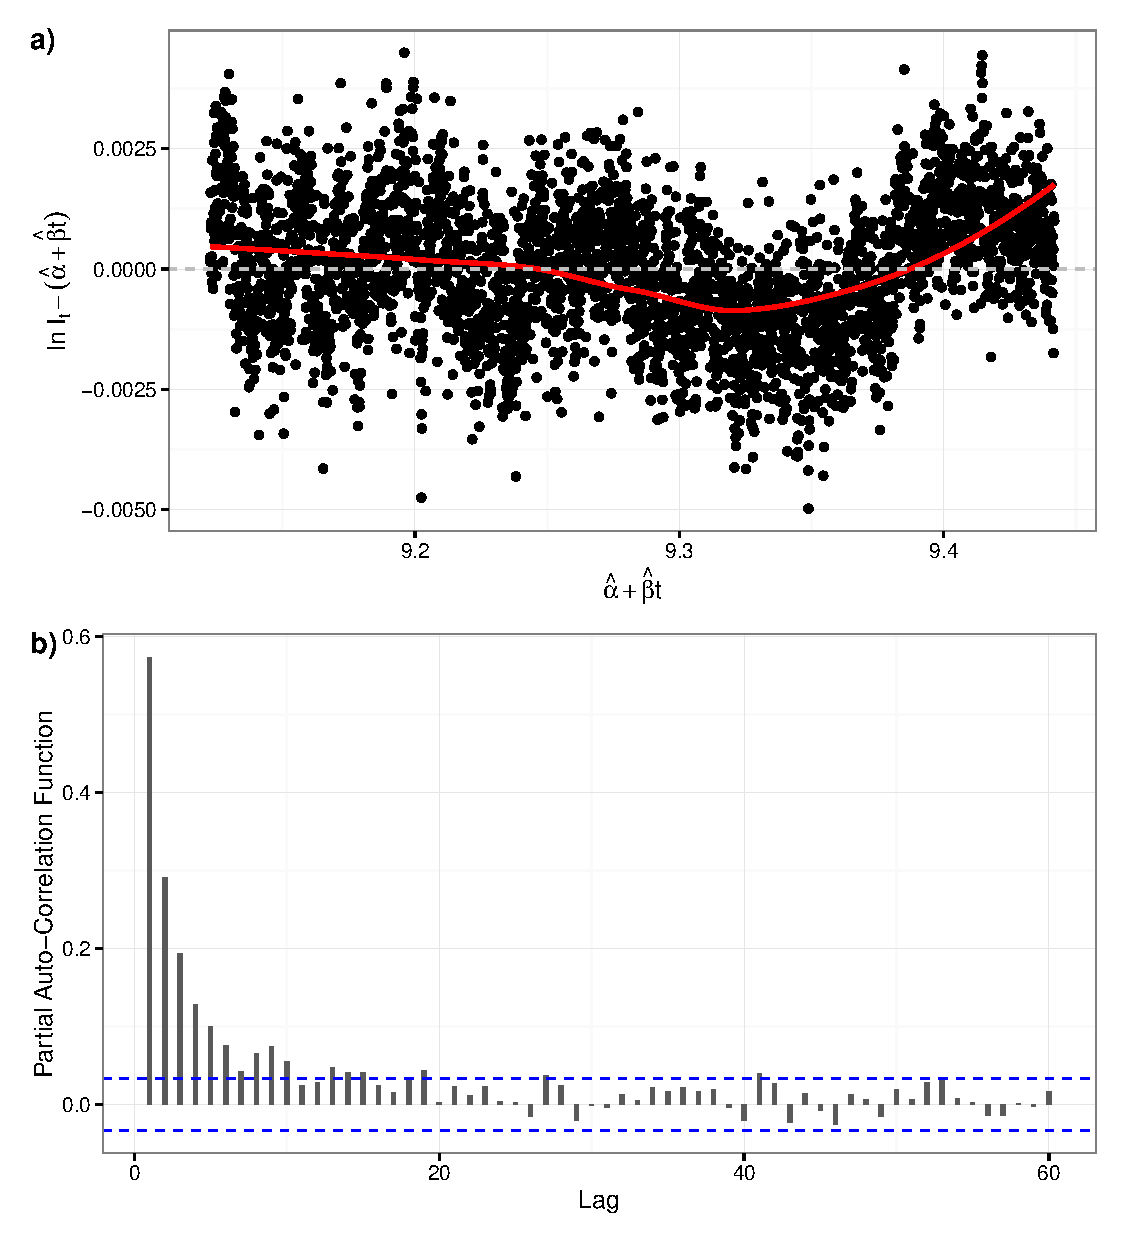
\includegraphics[scale=\scl]{img/DiagPlot_969.eps}
\caption{Some diagnostic plots for a typical 2016 cycle. a) The plot of the model residuals against the fitted values. The red line indicates that the linear model systematically underestimates the beam current at the cycle start and end, and overestimates it in mid-cycle. b) The plot of the partial correlation coefficients between the model residuals and lags of themselves. The dashed horizontal lines mark the 95\% confidence interval that the correlation is statistically insignificant.\label{fig:Run969}}
\end{figure}

\section{Effective cross section}
After the slopes are estimated from the raw measurement data, one can estimate the effective cross section. In this analysis, we used only the estimates from adjacent cycles, so as to minimize the effect of drifts of environmental variables such as target thickness (which is estimated to increase by $0.5~ \sfrac{\%}{\mathrm{hour}}$). The thickness by which the slope differences are divided, assumed constant, was provided by a Schottky measurement, made once during the experiment. Those estimates whose computation involved at least one slope which is deemed an outlier according to Tukey's range test are labeled unsound in TABLE~\ref{tbl:CS-all}. There are two outlier slopes in the 2012 experiment, and one in the 2016 experiment; all three are from target-off cycles. This may have been caused by problems with the target chopper, discovered during the 2016 experiment.

The effective cross section estimate's standard error (SE) is estimated by adding the squared standard errors of the paired slopes, not taking account of the covariance term. This is done so because depending on whether an on-slope is paired with the preceding or succeeding off-slope, the covariance term changes sign. Since there does not seem to be a reasonable criterion favoring either of the two mappings, the covariance term was omitted.

\section{Asymmetry}

The asymmetry was estimated as in equation~\eqref{eq:AyyEst}. In that expression, we used the target thickness as estimated using the Schottky measurements method~\cite{Stein} ($1.1\cdot 10^{14}$ cm$^{-2}$, measured once), and our own best estimate for the effective unpolarized cross section (411 mb, see TABLE~\ref{tbl:CS-all}).

\section{Results}
\begin{table}
\centering
\begin{threeparttable}
\caption{Cross section summary statistics. \label{tbl:CS-all}}
\begin{tabular}{c|llrcr}
\hline\hline
Year						& Soundness		& Closeness		& \#		& Mean\tnote{a} [a.u.]	& SE [a.u.] \\
\hline
\multirow{4}{*}{2012}		& Sound			& Close			& 4			& 507(507)				& 7  \\
							& Sound			& Far			& 8			& 553(563)				& 14 \\
							& Unsound		& Close			& 3			& 562(580)				& 36 \\
							& Unsound		& Far			& 5			& 515(512)				& 20 \\
							& All			& 				& 20		& 536(544)				& 10 \\
\hline					
\multirow{4}{*}{2016}		& Sound			& Close			& 40		& 409(411)				& 48 \\
							& Sound			& Far			& 92		& 396(385)				& 34 \\
							& Unsound		& Close			& 4			& 1400(1418)			& 170\\
							& Unsound		& Far			& 8			& 1453(1457)			& 69 \\
							& All			& 				& 144		& 486(473)				& 35 \\
\hline\hline
\end{tabular}
\begin{tablenotes}
\item[a] The value in parentheses is the variance-weighted mean.
\end{tablenotes}
\end{threeparttable}
\end{table}
\begin{figure}[h]
	\centering
	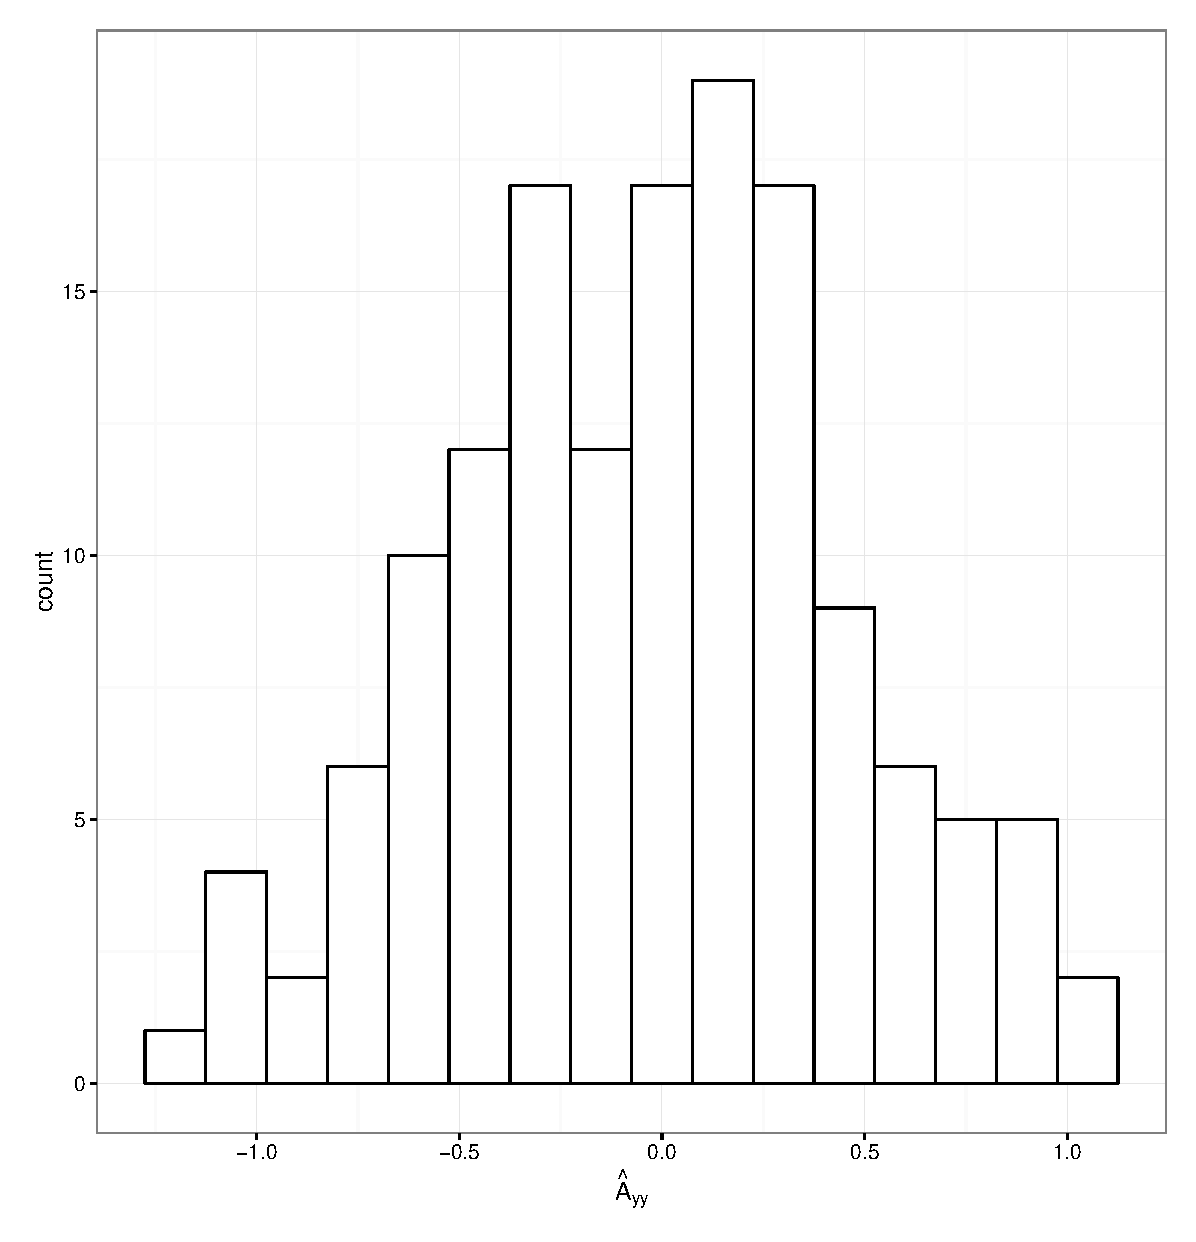
\includegraphics[scale=.35]{img/Ayy_dens.eps}
	\caption{Distribution of the Double-polarized cross section asymmetry estimate $\Ayy*$ in proton-deuteron scattering.\label{fig:AyyDensity}}
\end{figure}

Our best estimate for the effective $pp$ cross section is $\CS[0]^{pp} = 507 \pm 7$ a.u., that for the $pd$ reaction is $\CS[0]^{pd} = 411 \pm 48$. The asymmetry $\Ayy = \vp{(2 \pm 4)}{-2}$. The Quantile-Quantile plot shows that the estimate is distributed normally (see FIG.~\ref{fig:AyyDensity}); however the distribution's reduced chi-square $\chi^2_{red} = 7.8$. The upper limit of $\Ayy$ at the 95\% confidence level is 0.1.

There is a 31\% chance that our estimator of the asymmetry is zero in expectation. Considering that, as was explained in section~\ref{sec:Slope}, the slope means' dependence on the beam spin state is not statistically significant, we find it likely that this is the case. 

\section{Conclusion}

To improve the results, the following measures would be helpful:
\begin{inparaenum}
	\item a more frequent monitoring of the target thickness, to improve the effective cross section estimates;
	\item more stable vacuum conditions in the target chamber and also in the accelerator ring, which would help with the structural of the cycles;
	\item less variation in the CT offset, to avoid the introduction of an endogeneity bias; and also,
	\item more frequent polarimetry measurements, for the same reason as with the target thickness.
\end{inparaenum}

\begin{thebibliography}{9}
\bibitem{Conzett}
Homer E. Conzett, in Proceedings of the 7th International Conference on Polarization Phenomena in Nuclear Physics, Paris, France (1990).

\bibitem{Proposal}
P.D. Eversheim, B. Lorentz, and Yu. Valdau, Forschungszentrum J\"ulich, COSY, proposal \#215, 2012.

\bibitem{Weidemann}
Weidemann, C., F. Rathmann, H. J. Stein, B. Lorentz, Z. Bagdasarian, L. Barion, S. Barsov, et al. Phys. Rev. ST Accel. Beams \textbf{18}, 2 (2015).

%\bibitem{GaussMarkov}
%D.S.G. Pollock. 

\bibitem{Stein}
H. J. Stein, M. Hartmann, I. Keshelashvili, et al., Phys. Rev. ST Accel. Beams \textbf{11}, 052801 (2008).

\end{thebibliography}

\end{document}
